\documentclass[a4paper]{article}

\usepackage{pgfplots}

\begin{document}

\begin{tikzpicture}
%\tracingcommands=2\tracingmacros=2
	\begin{axis}[
		clip=false,
		symbolic x coords={A,B},
		xtick={A,B},
	]

	\addplot coordinates {(A,1) (B,2)};

	\node[pin={(A,1)}] at (normalized axis cs:0,1) {};

	\node[pin={(A,2)}] at (normalized axis cs:0,2) {};

	\node[pin={(middle,1)}] at (normalized axis cs:0.5,1) {};
		
	\end{axis}
\end{tikzpicture}

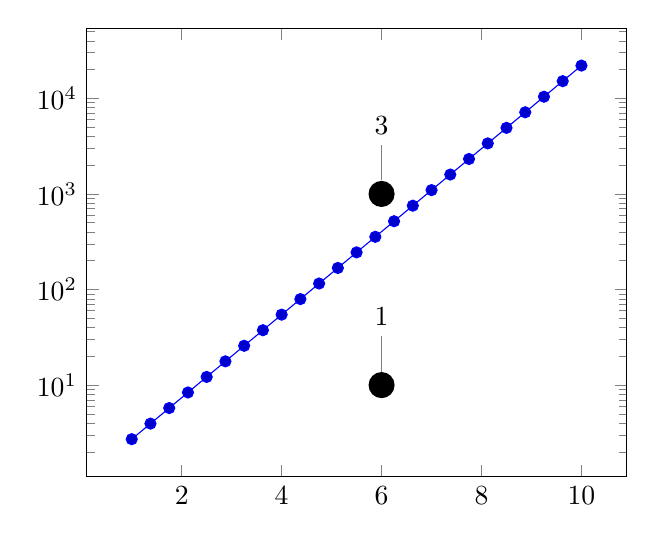
\begin{tikzpicture}
%\tracingcommands=2\tracingmacros=2
	\begin{semilogyaxis}[log basis y=10]
		
	\addplot+[domain=1:10] {exp(x)};

	\node[circle,fill,pin={1}] at (normalized axis cs:6,1) {};
	\node[circle,fill,pin={3}] at (normalized axis cs:6,3) {};

	\end{semilogyaxis}
\end{tikzpicture}
\end{document}

